\documentclass[aspectratio=169,hyperref={pdfpagelabels=false}]{beamer}
\input{preamble.tex}

\subtitle{\normalsize{Industrial IoT for Digitization of Electronic Assets}}
\title{Digital Twins \& Green Transition: An Introduction}

\setdepartment{DTU Wind and Energy System}
\setcolor{blue}

\begin{document}
\inserttitlepage

%B SLIDE 0
\begin{frame}{Agenda}
  \begin{itemize}
    \item The goals of the green transition.
    \item The European Targets.
    \item Future Projections in Denmark.
    \item Future Challenges.
    \item Digital Twins (DT): Some Definitions.
    \item Boosting the Digitalization with \textbf{DT}.
  \end{itemize}
\end{frame}

% SLIDE 1
\begin{frame}{}

  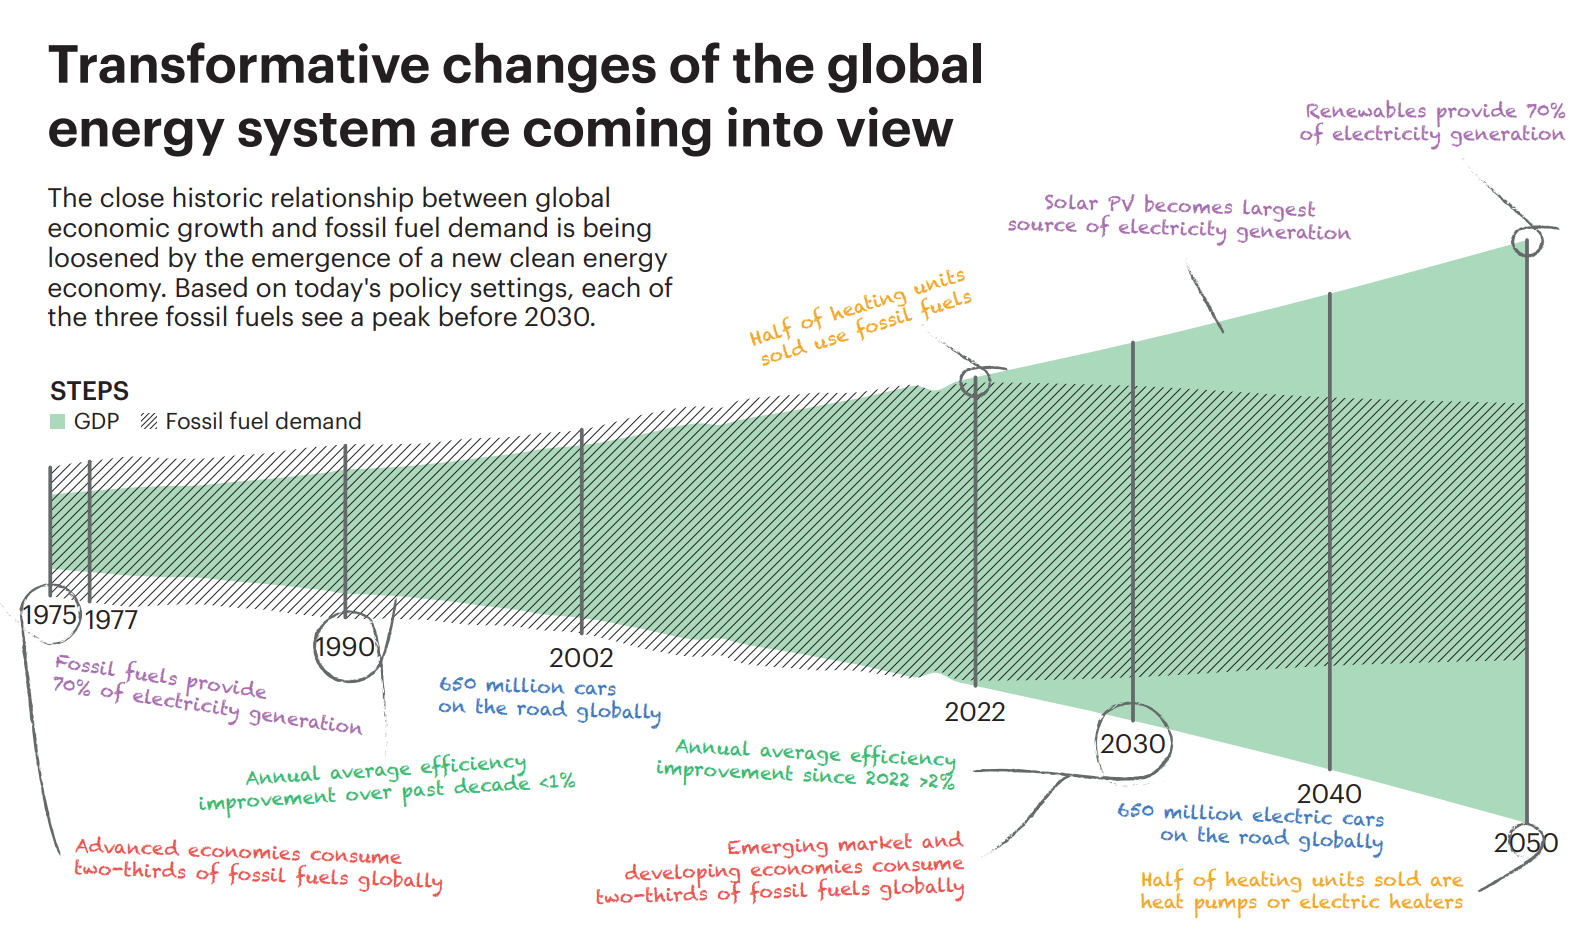
\includegraphics[width=0.9\textwidth]{img/pic0.png} 
  \let\thefootnote\relax\footnotetext{\tiny{World Energy Outlook 2023, iea}}
    \end{frame}

% SLIDE 2
    \begin{frame}{\Large{The Green Transition and European Targets}}
    Europe has set the goal of reducing 40\% of Greenhouse Gas emissions by 2030 and 80-95\% by 2050, to reach the target of maintaining global atmospheric warming below 2°\;C. 
    To accomplish this target, massive investment in renewable is on the way:

    \vspace*{1em}

        \begin{columns}
          % Left column
          \begin{column}{0.4\textwidth}
            % Add your text here
            \textbf{Key Goals: }
            \begin{itemize}
                \item[-] 45\% of Renewable resources by 2030
            \end{itemize}
            \begin{itemize}
                \item \textbf{600 GW} of Solar Capacity
                \item \textbf{450 GW} of Wind Capacity
            \end{itemize}
            
          \end{column}
      
          % Right column
          \begin{column}{0.7\textwidth}
            % Add your image here
            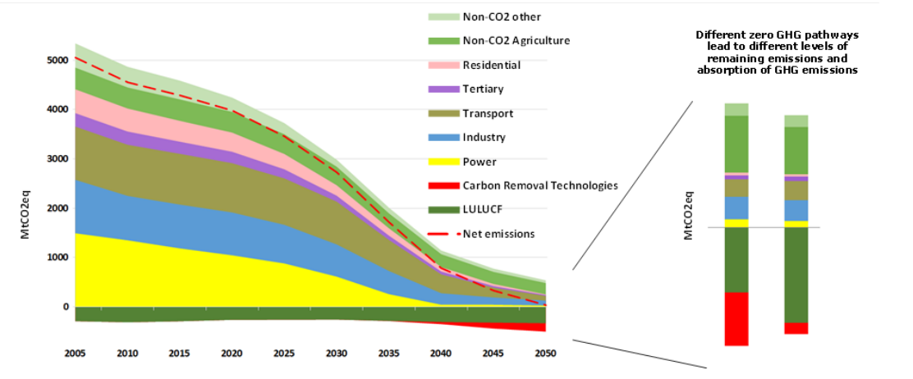
\includegraphics[width=\textwidth]{img/pic1.png} % Replace with your image path
          \end{column}
        \end{columns}
        \let\thefootnote\relax\footnotetext{\tiny{European policies on climate and energy towards 2020, 2030 and 2050}}
      \end{frame}

% SLIDE 3
\begin{frame}{\Large{Future Projections In Denmark}}

        \begin{columns}
          % Left column
          \begin{column}{0.4\textwidth}
            Word leading country in wind energy with more than 44\% of the energy production from renewable sources.
            Carbon Neutral by 2030, with Offshore and Onshore Wind up to 13 GW and Solar up to then 10 GW.
            
          \end{column}
      
          % Right column
          \begin{column}{0.5\textwidth}
            % Add your image here
            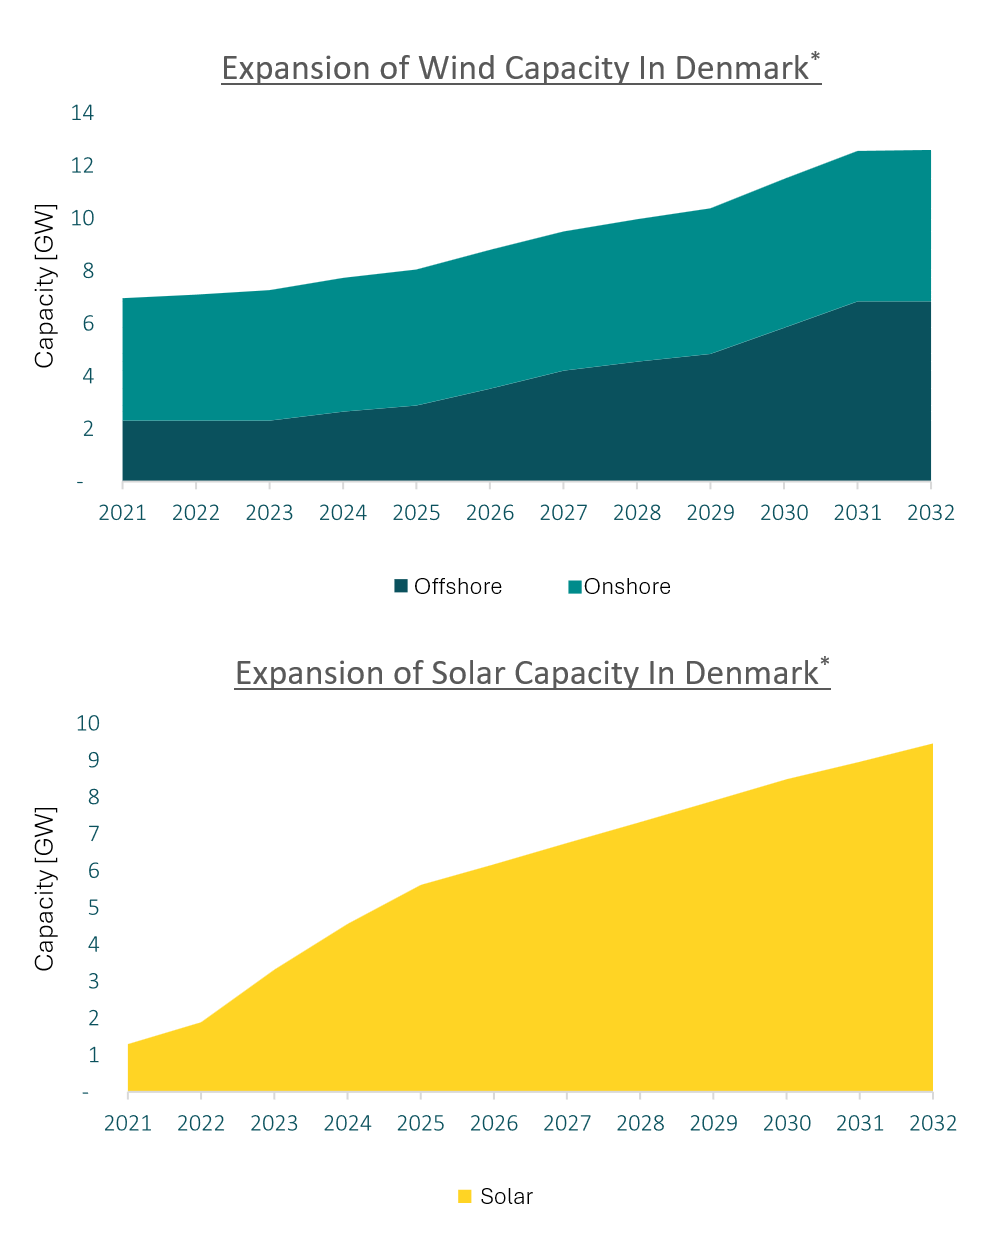
\includegraphics[width=0.75\textwidth]{img/pic2.png} 
          \end{column}
        \end{columns}
        \let\thefootnote\relax\footnotetext{\tiny{Energinet. (2022). SCENARIERAPPORT 2022 – 2032: Forventninger til fremtidens Systemydelser. Energinet}}
      \end{frame}

% SLIDE 4
\begin{frame}{}
  \begin{center}
  \Large{\textbf{What Are the Main Challenges of an Energy System Based on Renewables?}}
  \end{center}
  \vspace{1em}
  \begin{figure}[t]
    
\includegraphics[width=0.25\textwidth]{img/pic5.png} \centering
    \centering
    \end{figure}
  
\end{frame}
        
% SLIDE 5
\begin{frame}{\Large{Past and Future Challenges}}
  \begin{columns}
    % Left column
    \begin{column}{0.5\textwidth}
      \begin{itemize}
        \item Higher chance of frequency disturbances. 
        \item Higher capacity of Ancillary Services. 
        \item Tailored control strategies. 
        \item Optimize Storage and Production. \pause
      \end{itemize}
    \end{column}

    % Right column
    \begin{column}{0.5\textwidth}
      \begin{itemize}
        \item Exploit flexibility of variable loads (\textit{fans, drives, compressors}). 
        \item Aggregate multiple presumers.
        \item Data-driven modeling solutions. 
        \item Boosting digitalization in old energy assets. 
      \end{itemize}
    \end{column}
  \end{columns}
\end{frame}

\begin{frame}{\Large{Ancillary Services}}
\begin{figure}[h]
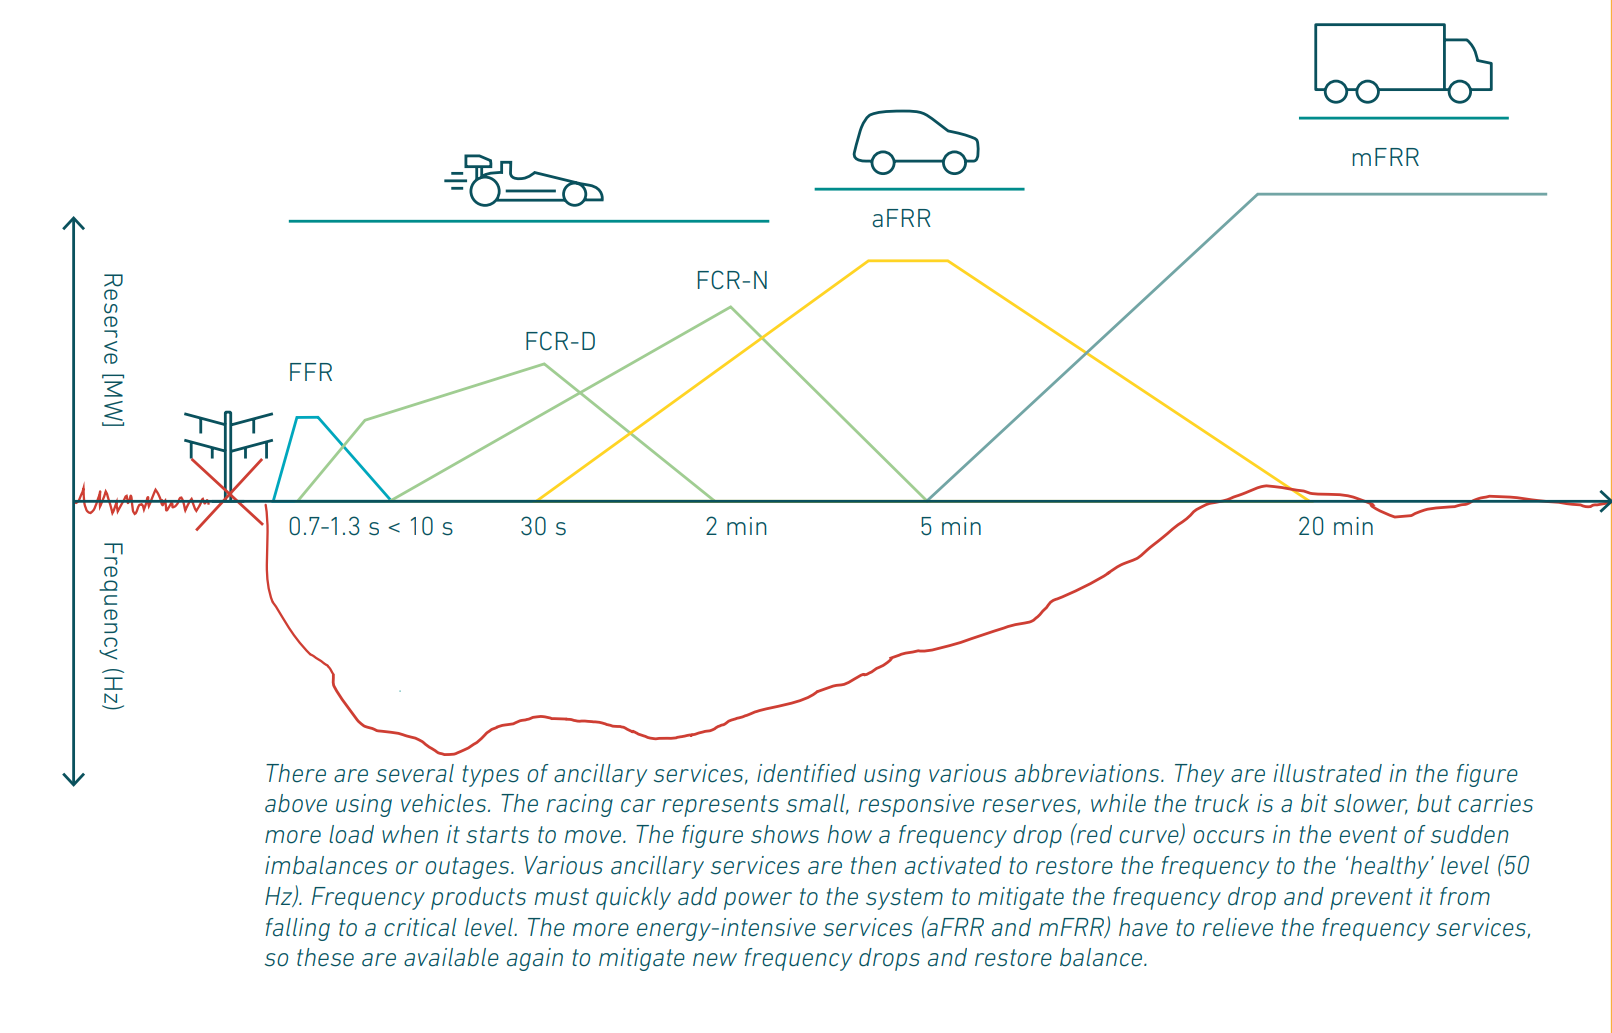
\includegraphics[width=0.80\textwidth]{img/ancillary_services.png} \centering
\let\thefootnote\relax\footnotetext{\tiny{Energinet - ANNUAL MAGAZINE 2023}}
\end{figure}
\end{frame}

% SLIDE 5
\begin{frame}{\Large{Digital Twins: Some Definitions}}
  \begin{figure}[h]
    \vspace{0em}
    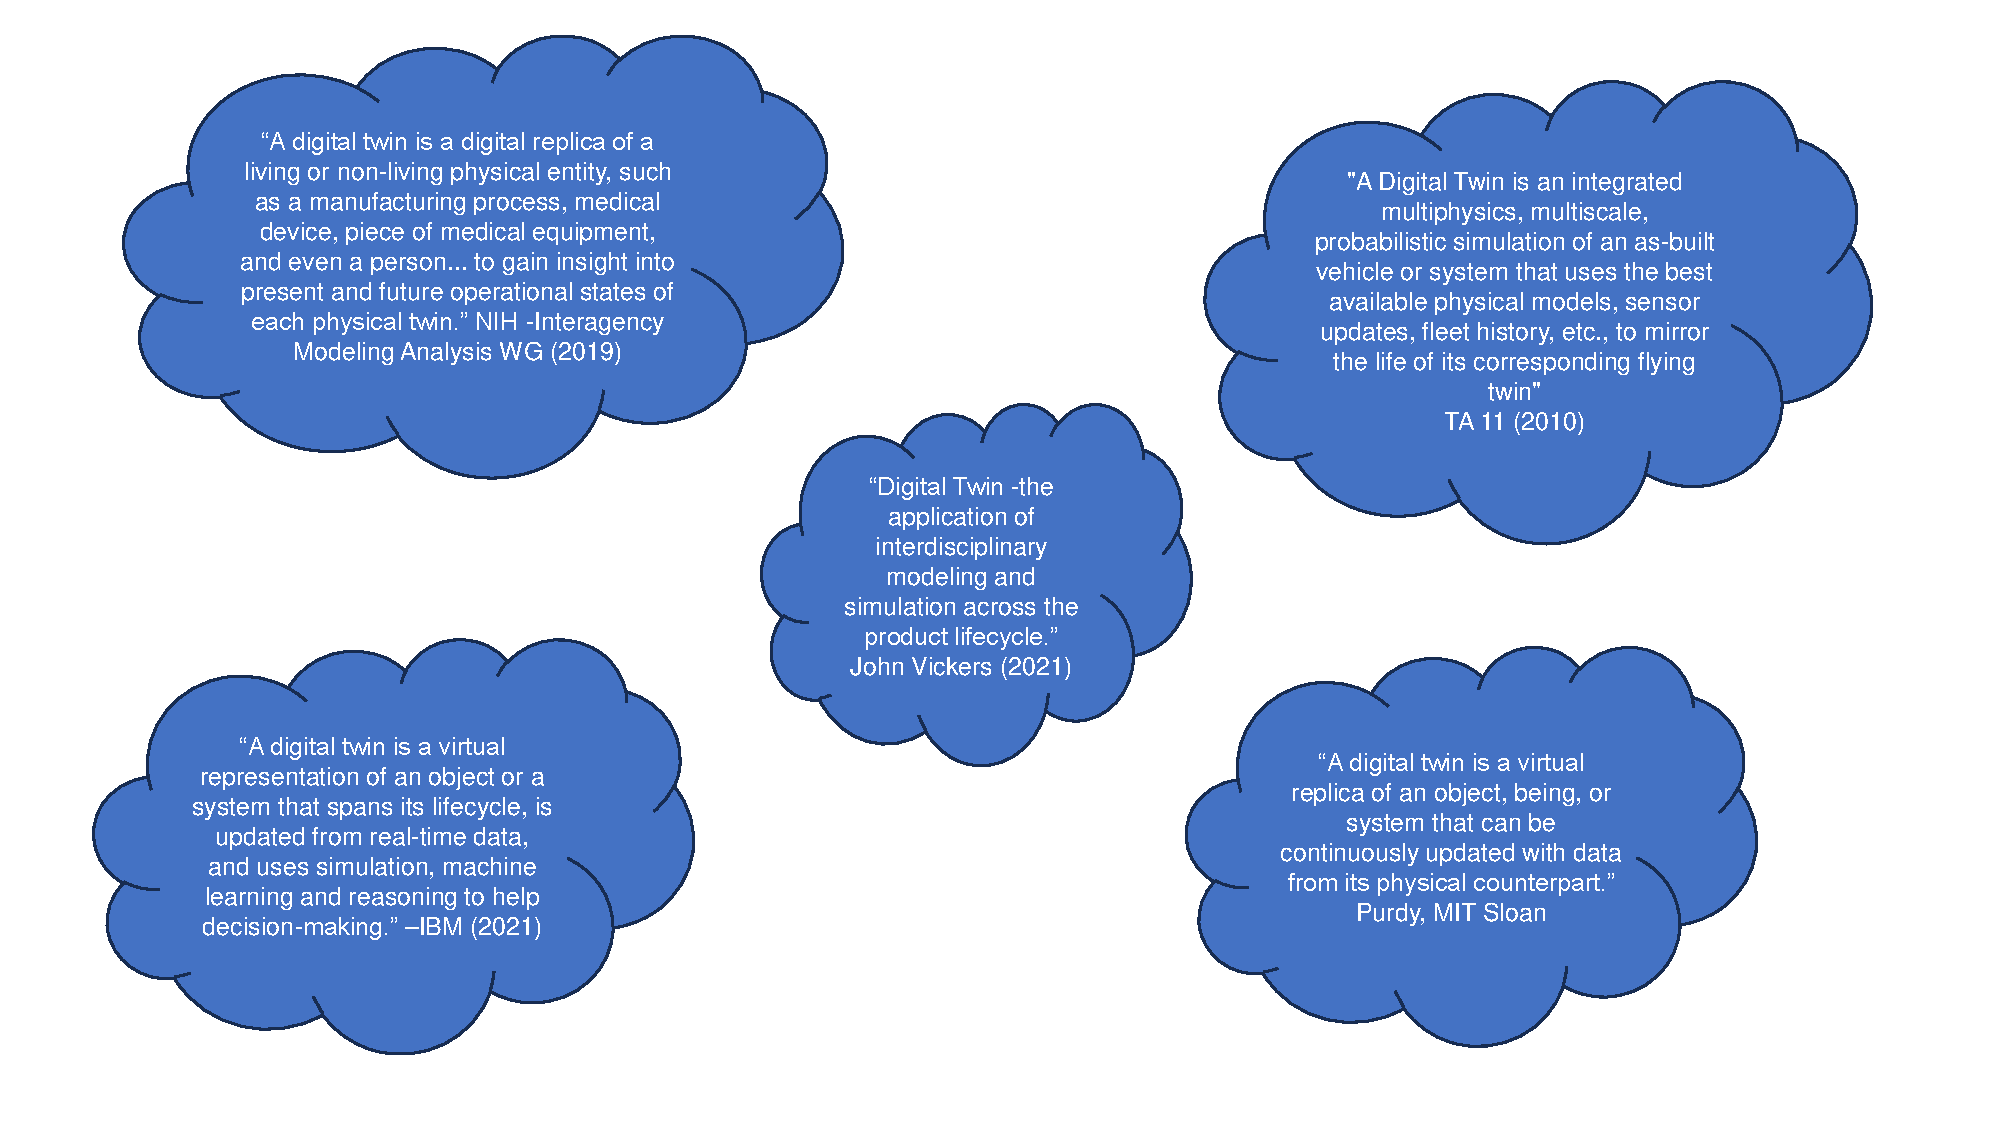
\includegraphics[width=1\textwidth]{img/digital_twin_definitions.pdf} \centering
  \end{figure}
\end{frame}

% SLIDE 6
\begin{frame}{\large{Digital Twins:} \\ \vspace{0.5em}
  \normalsize{A core technology to boost the Digitalization}}
\begin{figure}[h]
  \vspace{1em}
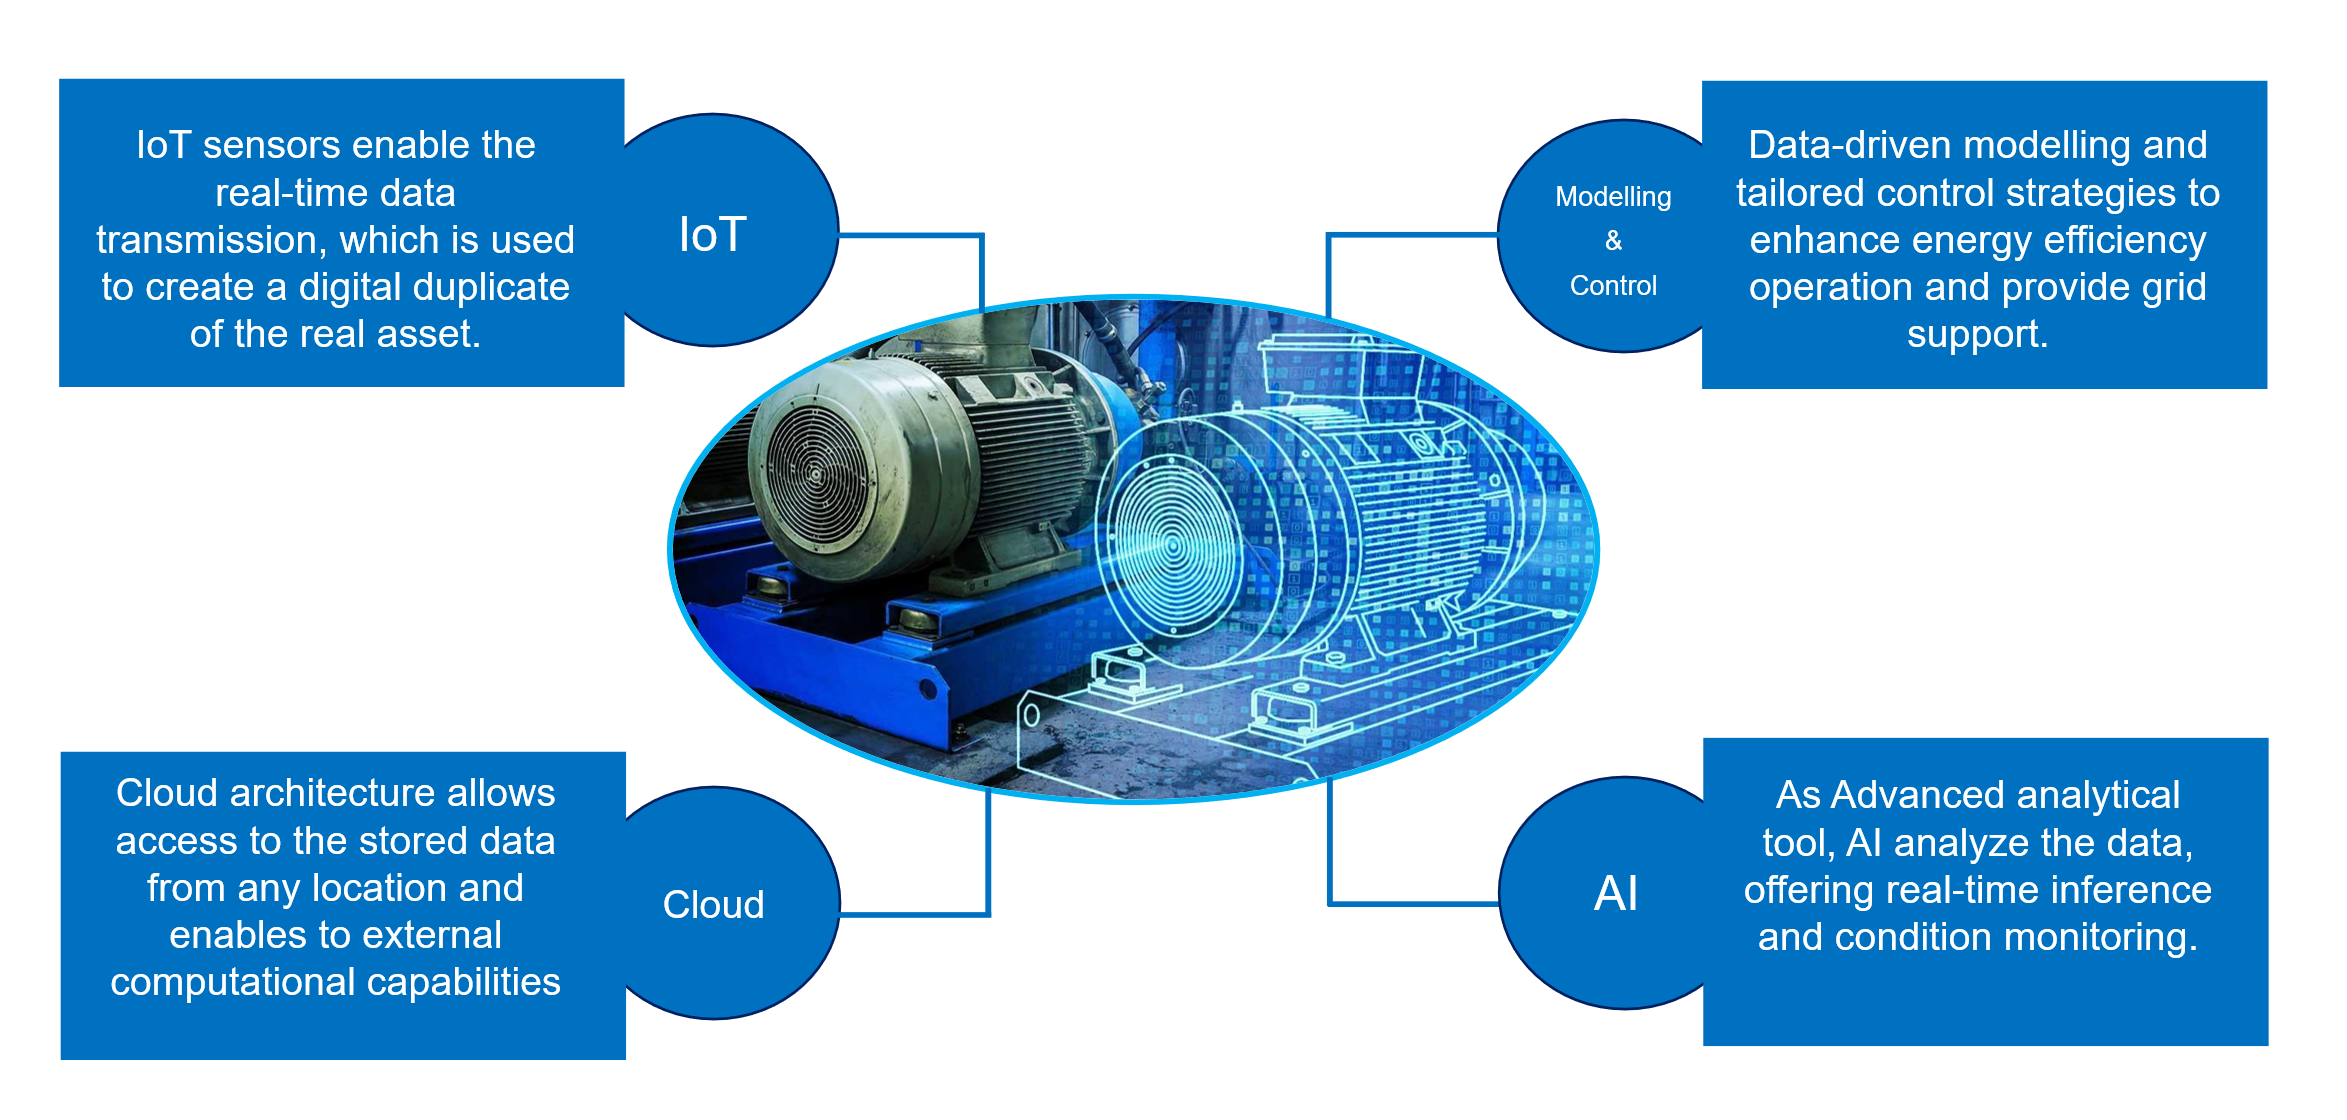
\includegraphics[width=1.05\textwidth]{img/pic7.png} \centering
\end{figure}
\end{frame}

% SLIDE 6
\begin{frame}{\large{Digital Twins:} \\ \vspace{0.5em}
  \normalsize{An application example to the Wastewater in Bornholm.}}
\begin{figure}[h]
  \vspace{1em}
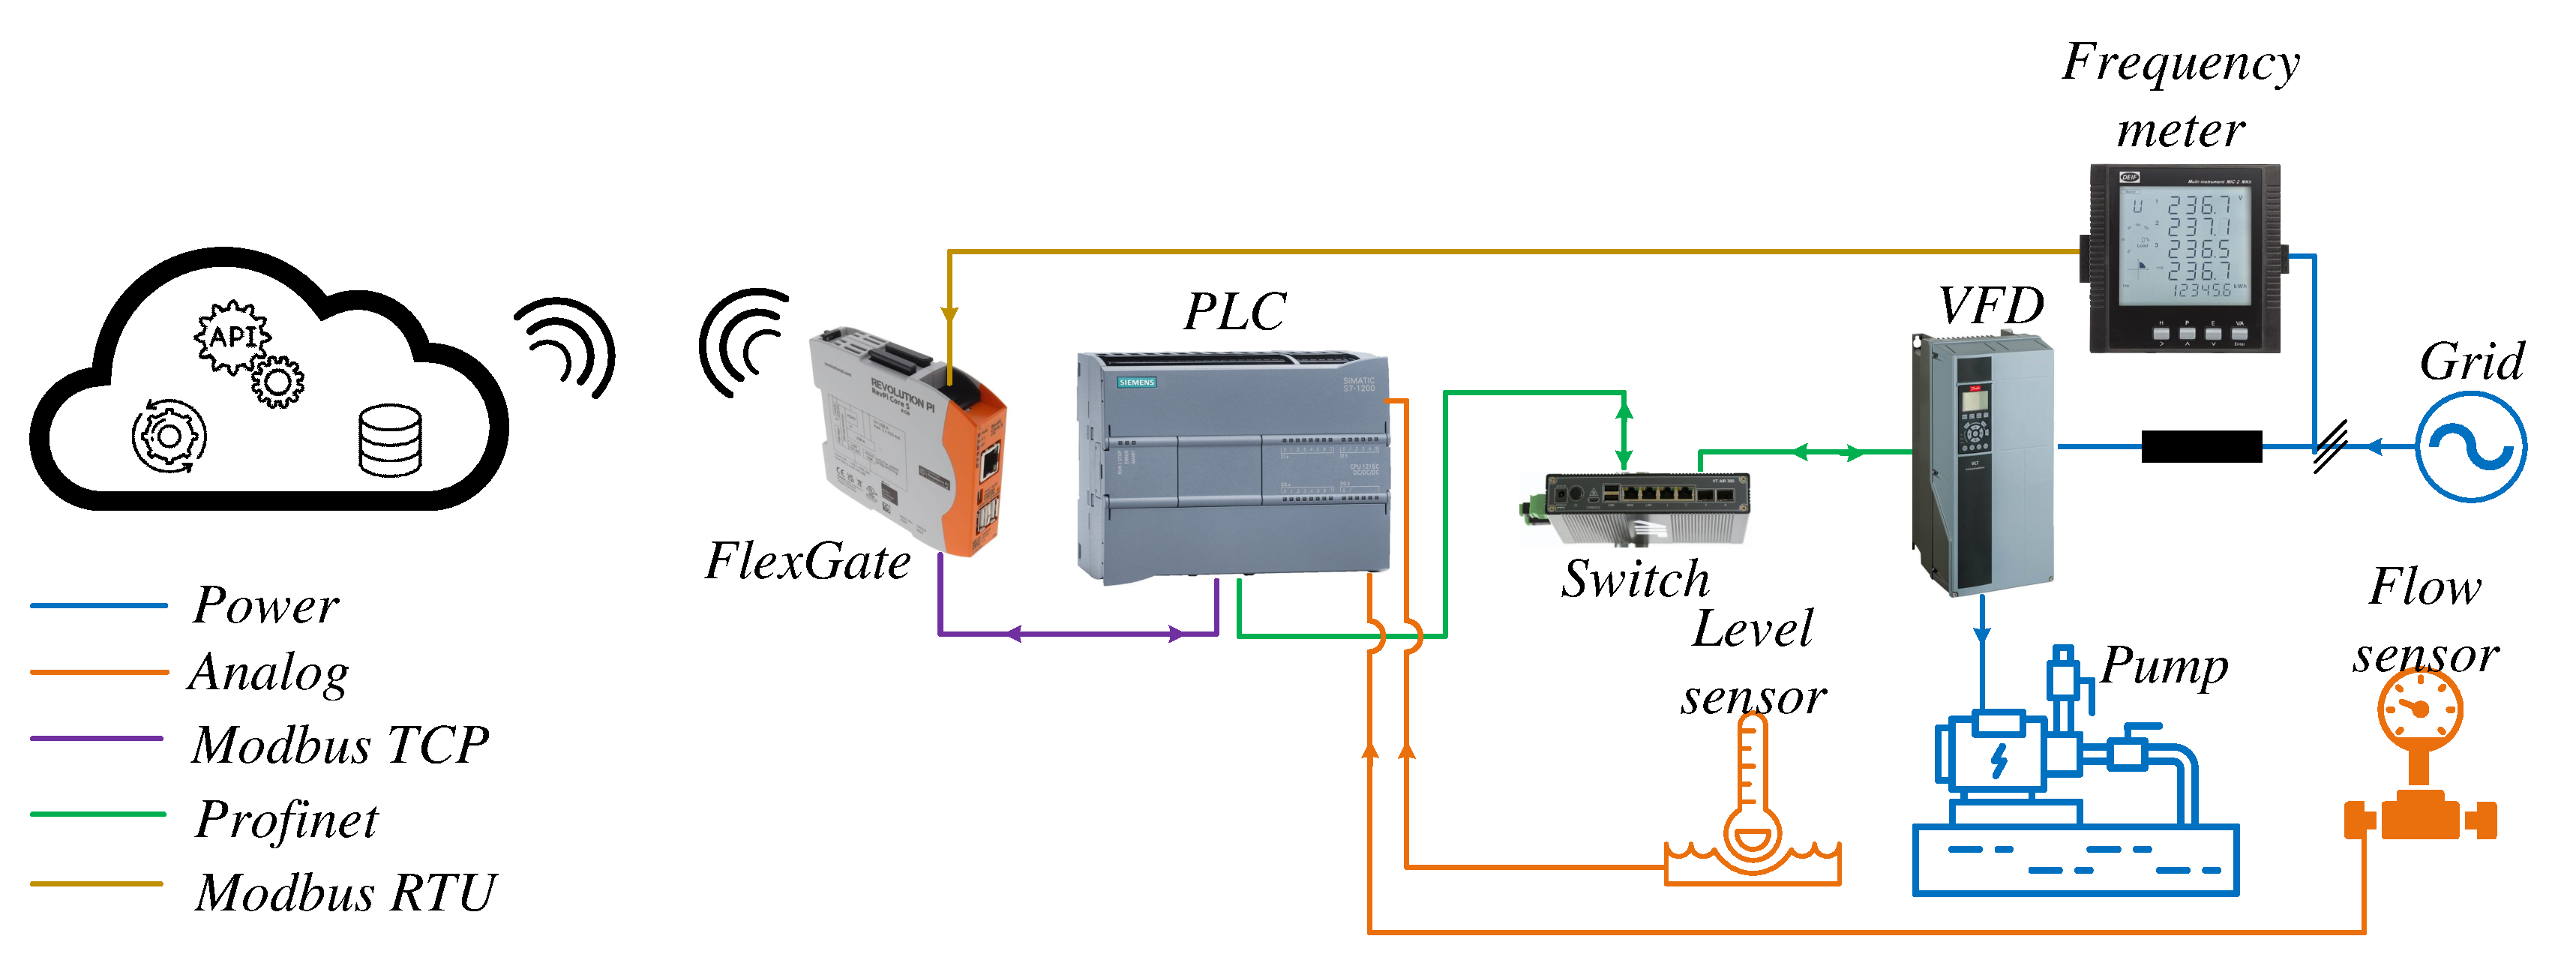
\includegraphics[width=0.95\textwidth]{img/Block_diagram_pump_ronne.pdf} \centering
\let\thefootnote\relax\footnotetext{\tiny{Quattrociocchi, A., Subroto, R. K., Oppedijk, W. M., \& Dragičević, T. (2023, October). 
Energy Efficiency Optimization of a Wastewater Pumping Station Through IoT and AI: A Real-World Application of Digital Twins.}}
\end{figure}
\end{frame}

\end{document}